\documentclass{article}
\usepackage{qilin}
\tikzstyle{process} = [rectangle, rounded corners, minimum width=1.5cm, minimum height=0.5cm,align=center, draw=black, fill=gray!30, auto]
\title{AER372: Control Systems  \\ Assignment 4}
\author{QiLin Xue}
\date{Spring 2023}

\usepackage{empheq}
\newcommand*\widefbox[1]{\fbox{\hspace{2em}#1\hspace{2em}}}

\usepackage{mathrsfs}
\usetikzlibrary{arrows}
\usepackage{stmaryrd}
\usepackage{accents}
\newcommand{\ubar}[1]{\underaccent{\bar}{#1}}
\usepackage{pgfplots}
% \numberwithin{equation}{section}
\usepackage{amsmath, amssymb, graphics, setspace}

\newcommand{\mathsym}[1]{{}}
\newcommand{\unicode}[1]{{}}
\usepackage{tabu}
\newcounter{mathematicapage}
\usepackage[numbered,framed]{matlab-prettifier}

\usepackage{filecontents}
\let\ph\mlplaceholder % shorter macro
\lstMakeShortInline"

\lstset{
  style              = Matlab-editor,
  basicstyle         = \mlttfamily,
  escapechar         = ",
  mlshowsectionrules = true,
}

\begin{document}

\maketitle
\begin{enumerate}[label=\textbf{4.\arabic*}]
\item Recall that a lead compensator is in the form of 
\begin{equation}
    D_c(s) = K\frac{Ts+1}{\alpha Ts + 1}
\end{equation}
for $z < p.$ Our transfer function is 
\begin{equation}
    G(s) = \frac{50000}{s(s+10)(s+50)},
\end{equation}
and we wish to satisfy $PM > 50^\circ$ and $\omega_{BW} \ge 20\text{ rad/sec}.$ The Bode Plot is shown below for the original system with no compensator,
\begin{center}
    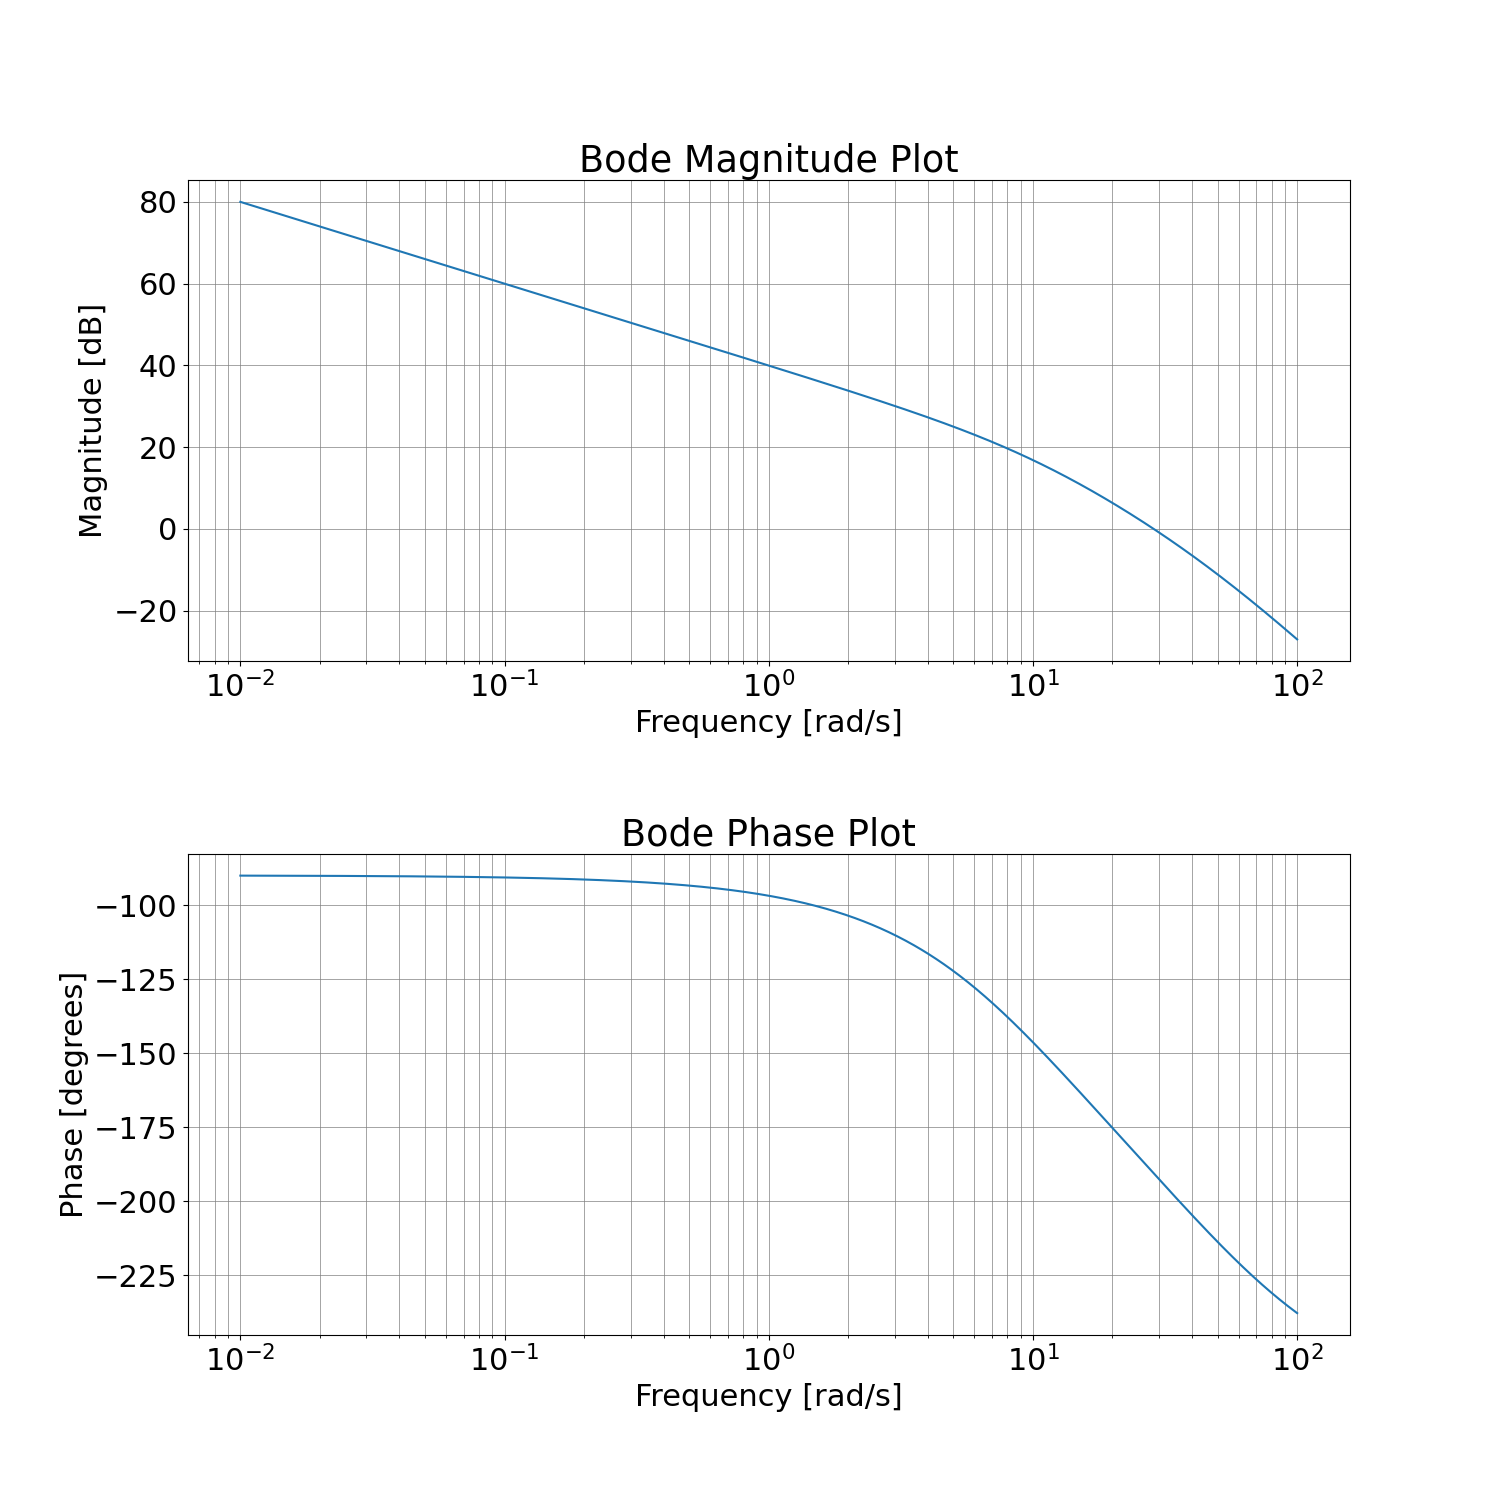
\includegraphics[width=0.7\linewidth]{A4_imgs/q1_bode_nothing.png}
\end{center}
which has the following parameters (see Appendix for computation)
\begin{align}
    \omega_{BW} &= 33.61 \text{ rad/s} \\
    \omega_C &= 28.74 \text{ rad/s}\\
    PM &= -10.70^\circ
\end{align}
\begin{enumerate}[label=(\arabic*)]
    \item Note that $K=1/10$ gives $w_C = 7.83 \text{ rad/s}.$
    \item From above, we have $PM=-10.7^\circ$
    \item Set requirement to be $PM \ge 50^\circ + 10^\circ$ instead, so 
    \begin{equation}
        PM = 60^\circ - (10.7^\circ) = 70^\circ = \phi_\text{max}
    \end{equation}
    \item Compute 
    \begin{equation}
        \alpha = \frac{1-\sin\phi_\text{max}}{1+\sin\phi_\text{max}} = 0.031
    \end{equation}
    \item Pick $\omega_\text{max}=20$ to get 
    \begin{equation}
        T_d = \frac{1}{\sqrt{\alpha} \omega_\text{max}} = 0.283980917
    \end{equation}
    so 
    \begin{equation}
        D_c(s) = \frac{0.28s+1}{0.0088s+1}.
    \end{equation}
    This gives the following Bode Plot,
    \begin{center}
        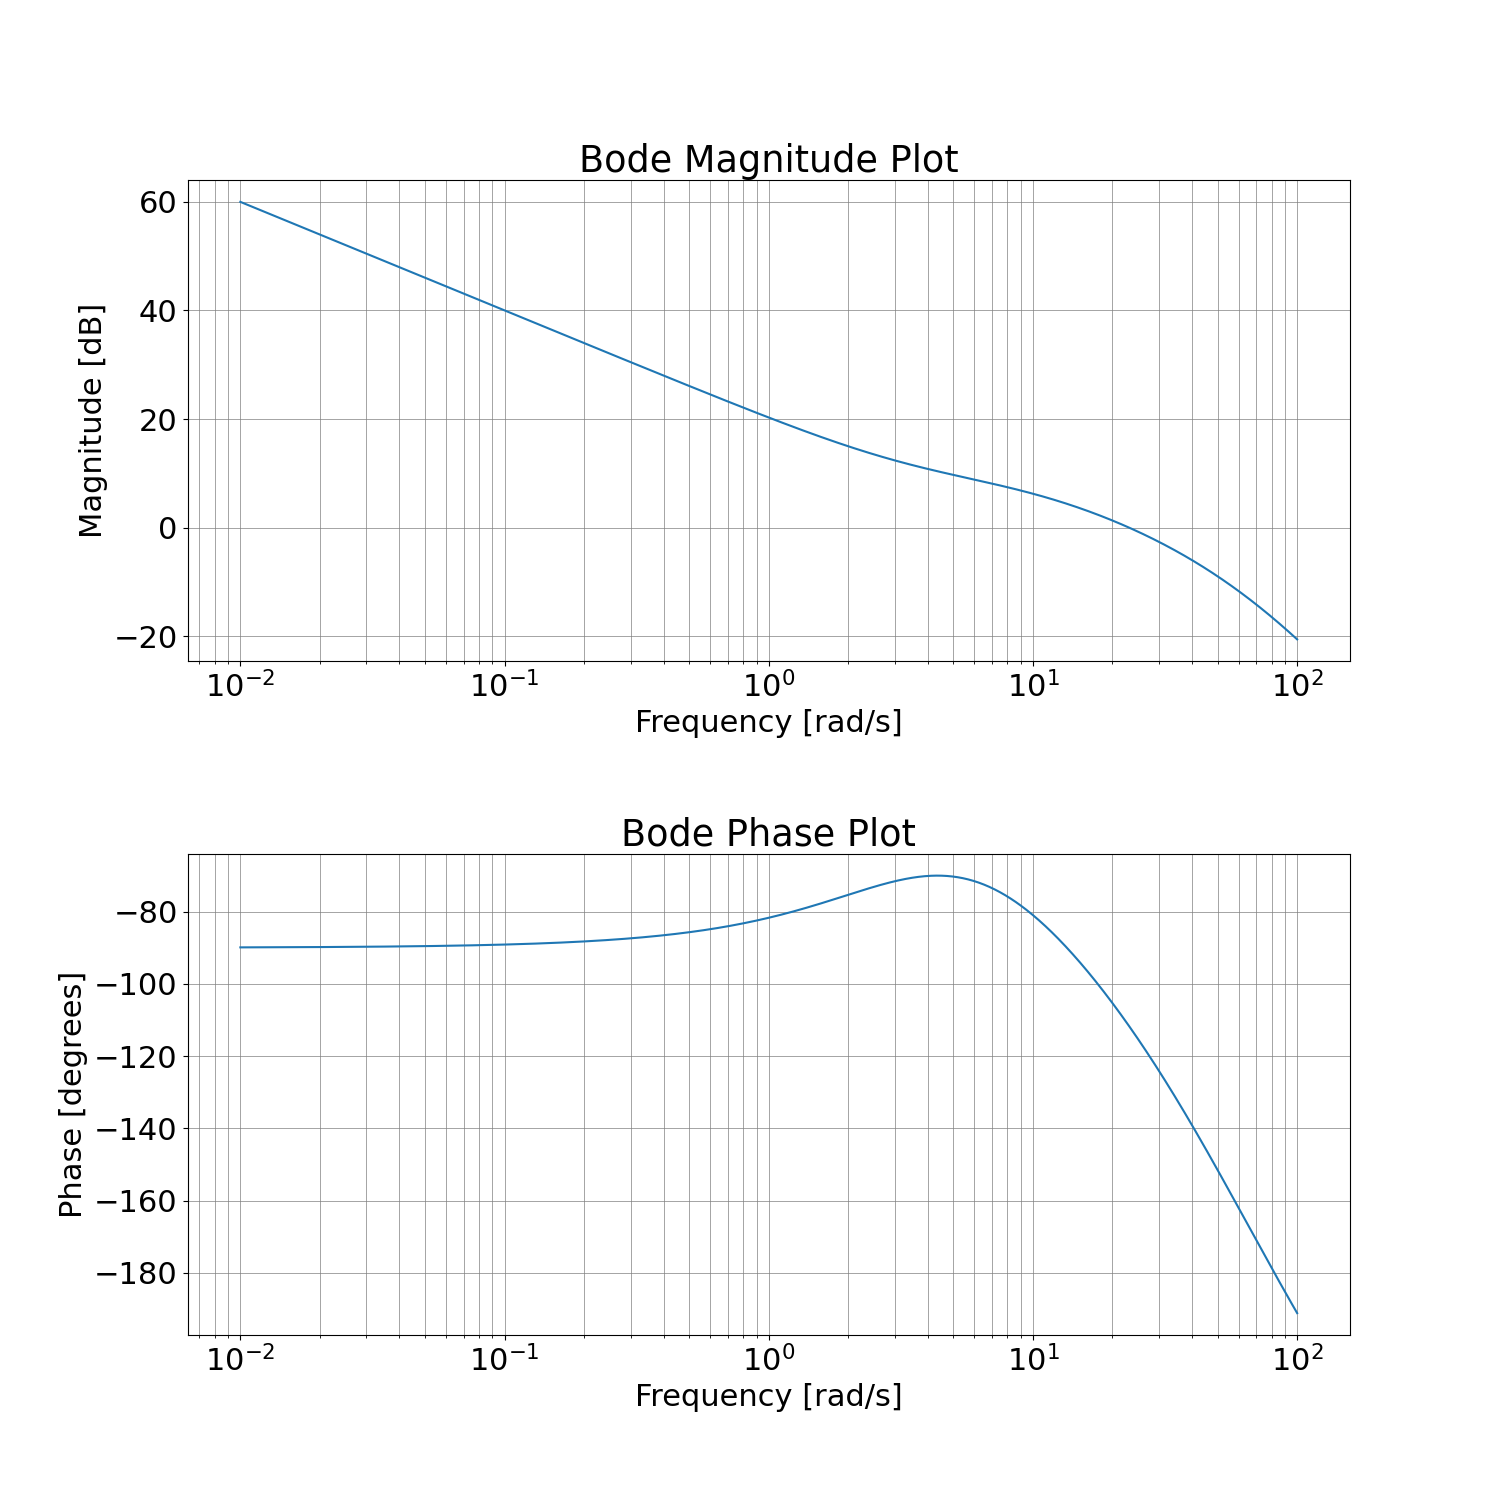
\includegraphics[width=0.7\linewidth]{A4_imgs/q1_bode_final.png}
    \end{center}
    which has parameters 
    \begin{align}
        \omega_{BW} &= 31.22 \text{ rad/s} \\
        \omega_C &= 23.25 \text{ rad/s}\\
        PM &= 68.04^\circ
    \end{align}
    which satisfies the necessary conditions. The bandwidth is around 
    \begin{equation}
        \omega_{BW} \approx 1 \text{ rad/s}.
    \end{equation}
\end{enumerate}
\newpage
\item A lag compensator is in the form 
\begin{equation}
    D_c(s) = K \alpha \frac{T_Is+1}{\alpha T_Is + 1}
\end{equation}
for $\alpha > 1.$ For unity DC gain, we want $D_c(0)=1$ so $K=\frac{1}{\alpha}.$ The frequency response for 
\begin{equation}
    G(s) = \frac{10}{s(s/1.4+1)(s/3+1)} = \frac{210}{s (s + 3) (5 s + 7)} = \frac{210}{5 s^{3} + 22 s^{2} + 21 s}
\end{equation}
looks like the following,
\begin{center}
    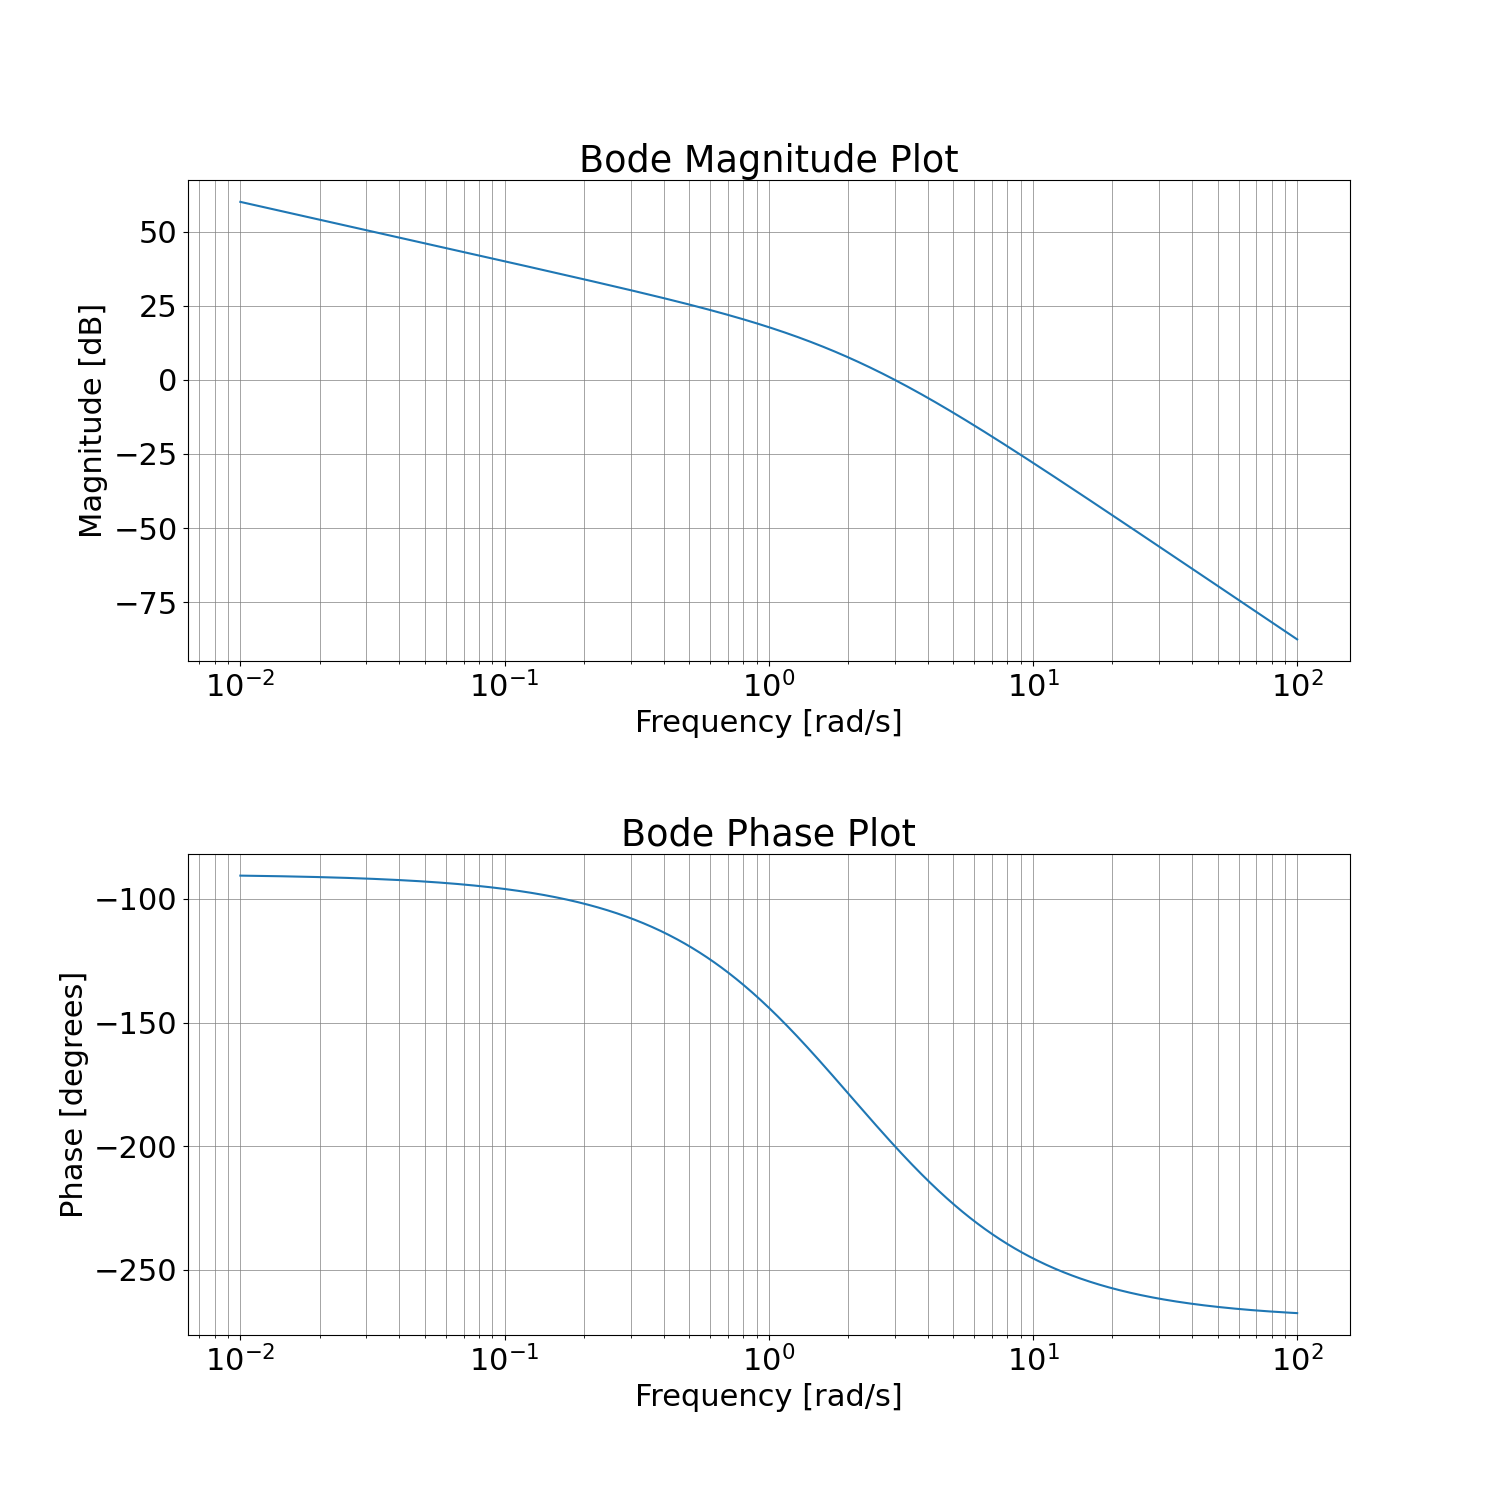
\includegraphics[width=0.7\linewidth]{A4_imgs/q2_bode_nothing.png}
\end{center}
which has parameters
\begin{align}
    \omega_{BW} &= 3.48 \text{ rad/s} \\
    \omega_C &= 3.00 \text{ rad/s}\\
    PM &= -20.02^\circ
\end{align}
To design our controller, we first assume that adding in the compensator will not significantly change the shape of the phase plot. The frequency at which the phase margin is $45^\circ$ (where we added $10^\circ$ for safety) is $\omega_0 = 0.81\text{ rad/s}.$ The magnitude at this frequency is 
\begin{equation}
    M_0 = 20\text{ dB},
\end{equation}
so we need to determine $\alpha,T$ such that 
\begin{equation}
    |D_c(j\omega_0)|= 10^{-20/20} = 0.1.
\end{equation}
The magnitude at high frequencies approach
\begin{equation}
    \lim_{x \to \infty} |D_c(xj)| = \frac{1}{\alpha},
\end{equation}
so set $\alpha = 10$ and pick the corner frequency to be 
\begin{equation}
    1/T_I = 0.81/10 = 0.081\text{ rad/s}
\end{equation}
so we know that at $\omega_0 = 0.81\text{ rad/s}$, we can guarantee that the magnitude is $0\text{ dB}.$ From the above equation, we get $T_I = 12.3$ so we get our first estimate of 
\begin{equation}
    D_c(s) = \frac{12.3s+1}{123s+1}.
\end{equation}
The new Bode Plot is shown below,
\begin{center}
    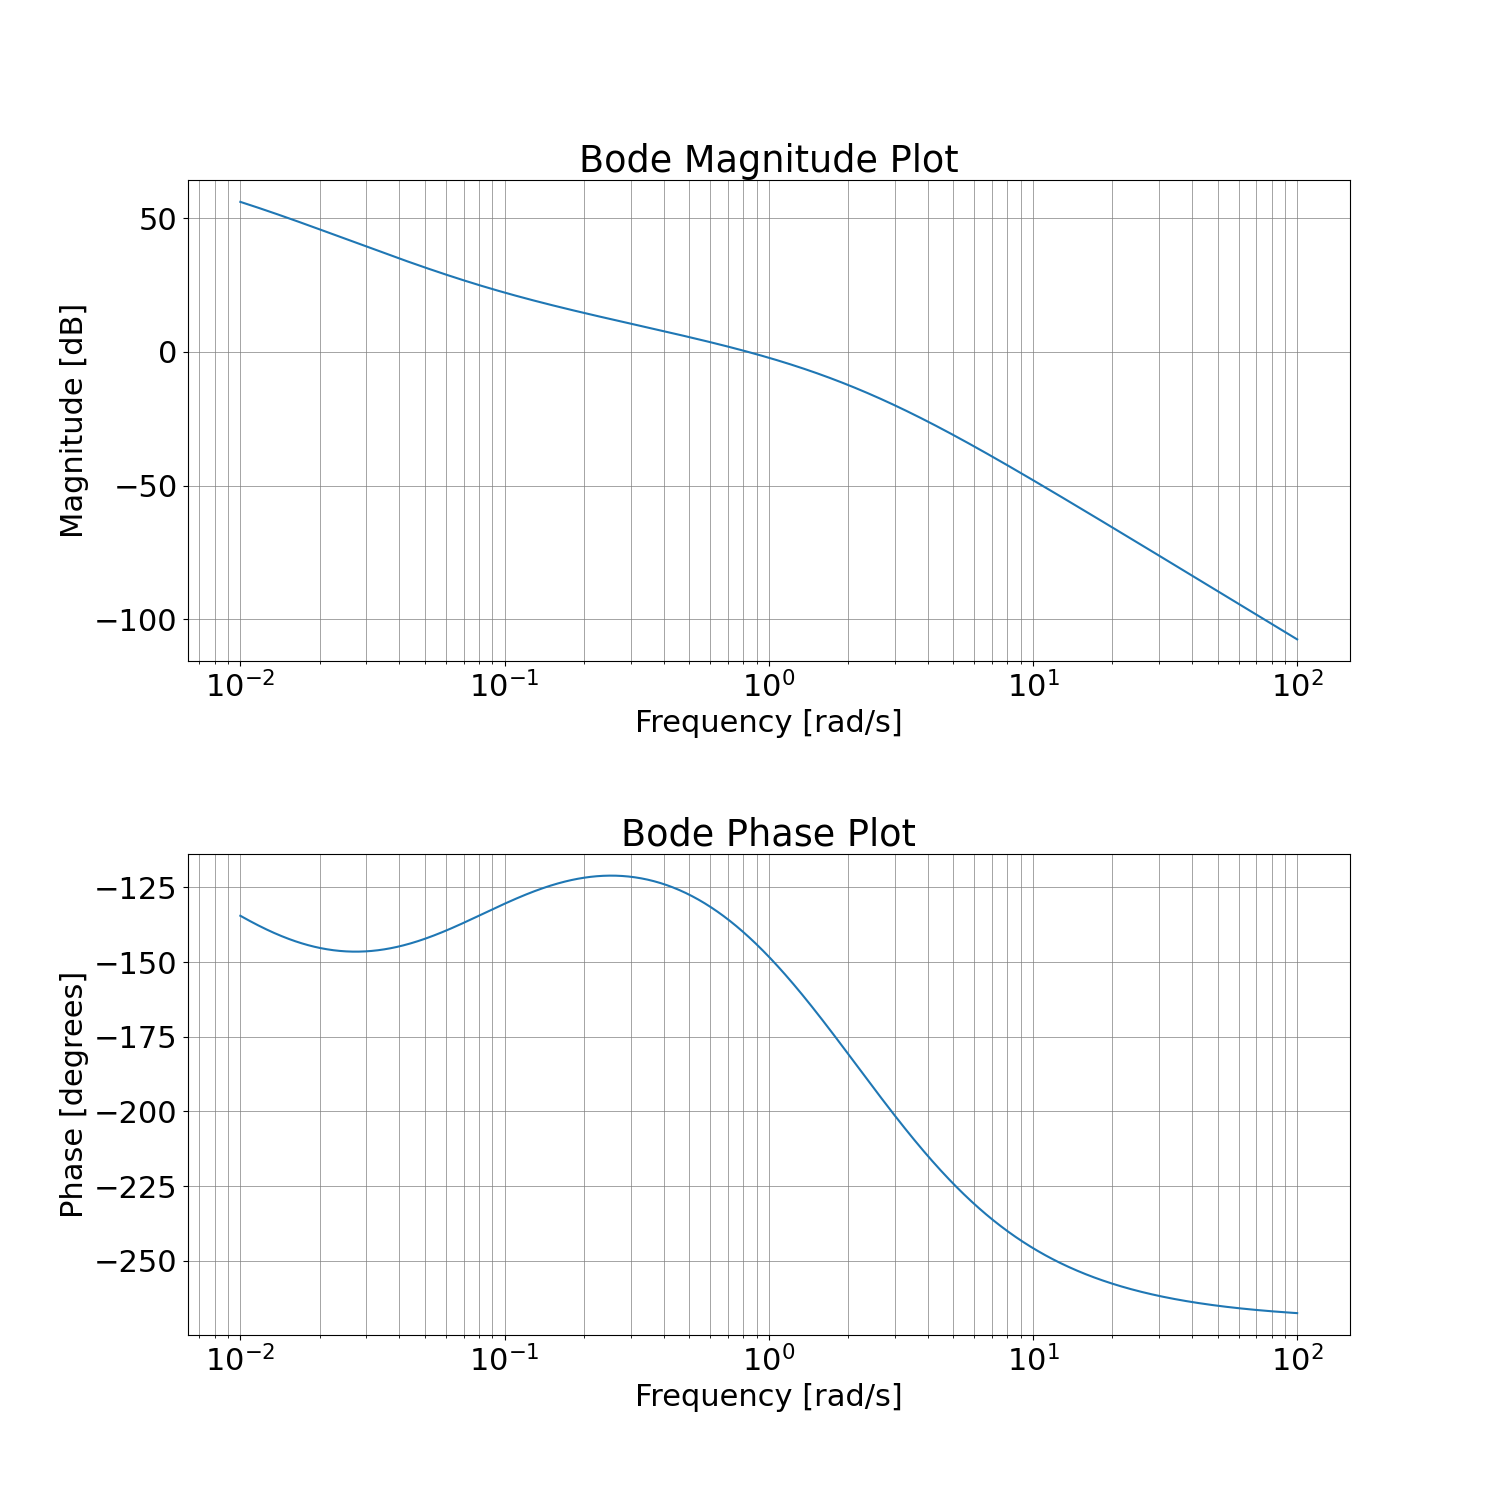
\includegraphics[width=0.7\linewidth]{A4_imgs/q2_bode_final.png}
\end{center}
which has 
\begin{equation}
    PM = 38.61^\circ,
\end{equation}
thus satisfying the necessary conditions.
\newpage
\item We have 
\begin{equation}
G(s) = \frac{0.05(s+25)}{s^2(s^2+0.1s+4)}  = \frac{s + 25}{20 s^{4} + 2 s^{3} + 80 s^{2}}
\end{equation}
which has the following Bode Plot,
\begin{center}
    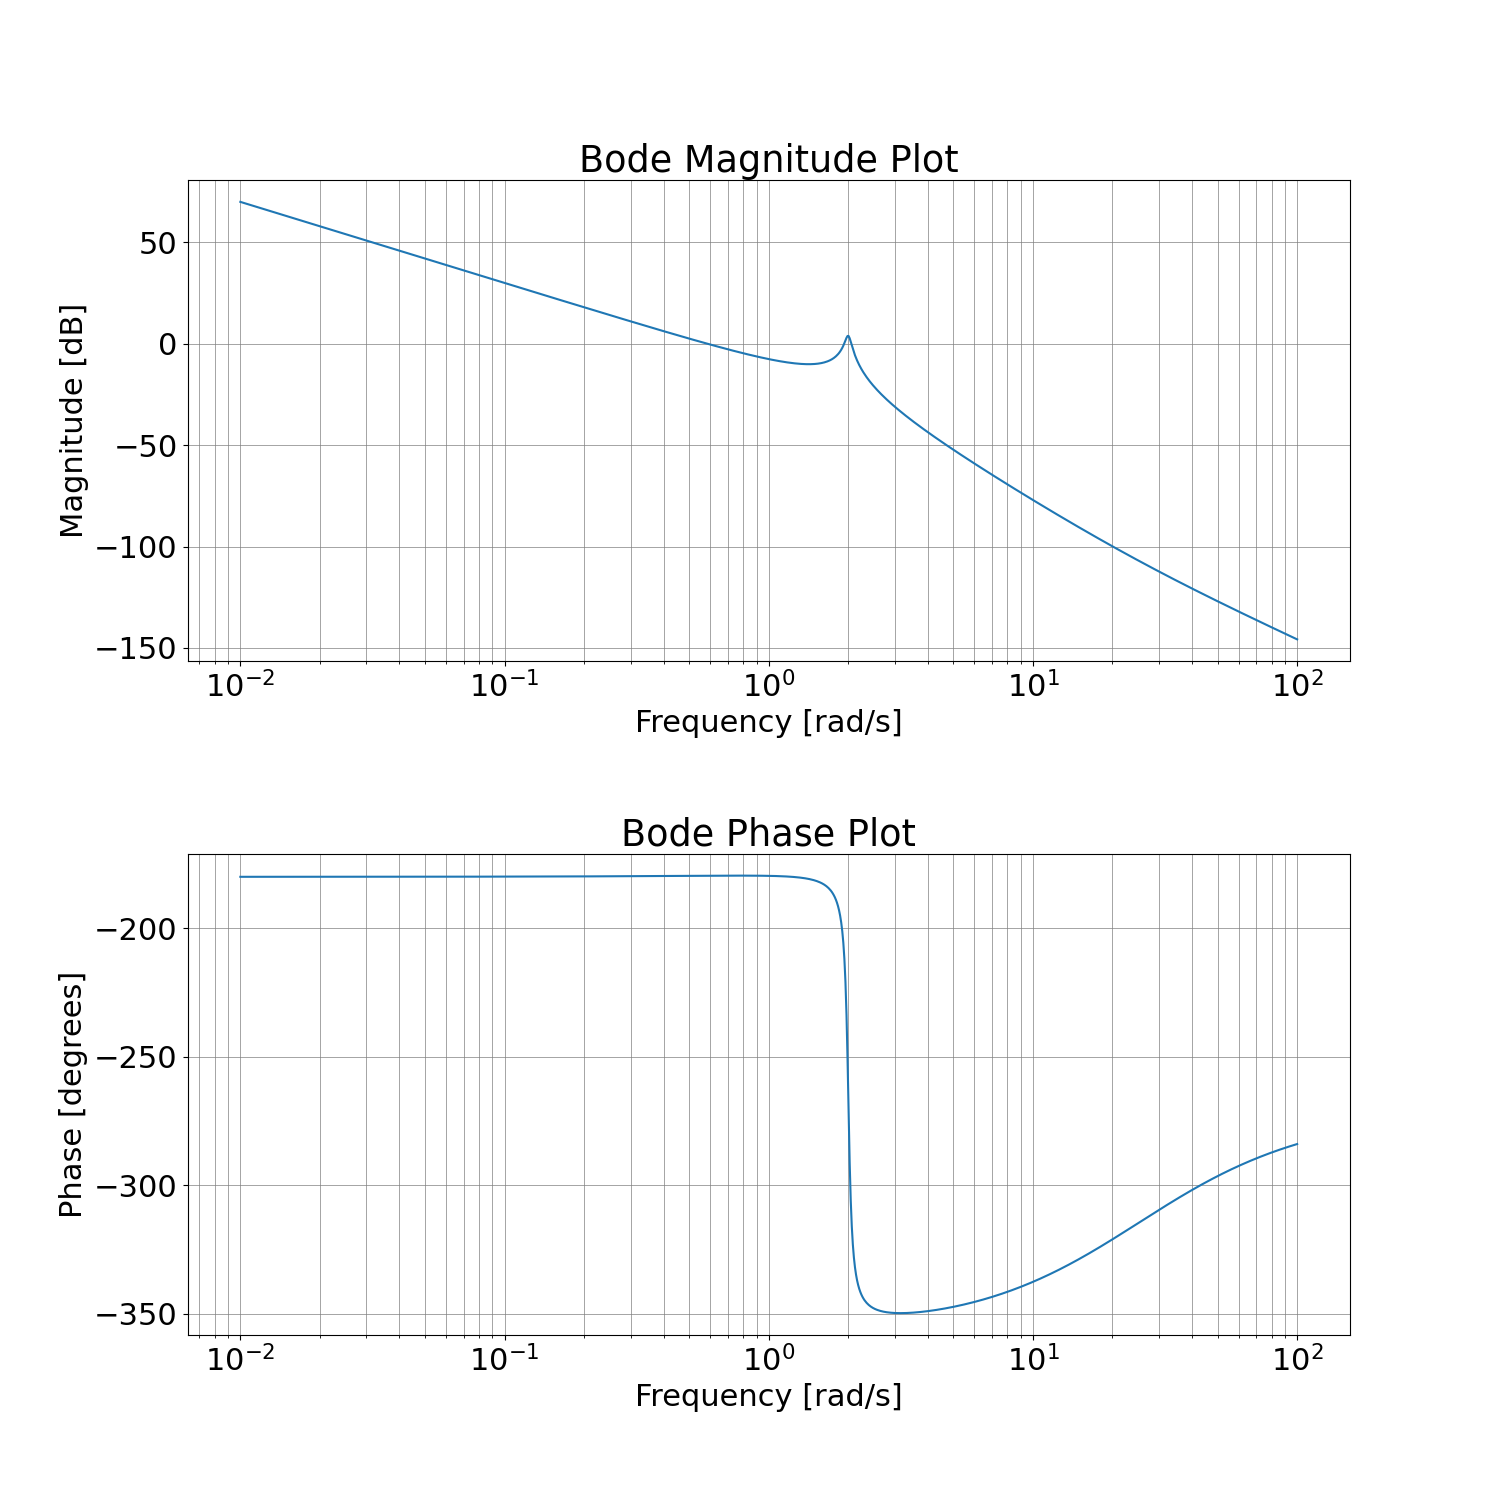
\includegraphics[width=0.7\linewidth]{A4_imgs/q3_bode_nothing.png}
\end{center}
% w_BW = 0.71 rad/s
% w_C = 0.59 rad/s
% PM = 0.43 degrees
% GM = 9.57
and has the following parameters
\begin{align}
    \omega_{BW} &= 0.71 \text{ rad/s} \\
    \omega_C &= 0.59 \text{ rad/s}\\
    PM &= 0.43^\circ \\ 
    GM &= 9.57.
\end{align}
The condition for GM is already satisfied, but we want $PM \ge 45^\circ.$ Let us considder different compensations:
\begin{itemize}
    \item Lag Compensator: We can increase the gain at low frequencies and decrease the gain at high frequencies. Therefore, if we want to increase the phase margin, we are also decreasing the bandwidth!
    \item PI Compensator: Similar to above, this is designed to keep the bandwidth low by increasing the gain at low frequencies and decreasing the gain at high frequencies, except now the gain approaches infinity as the frequency approaches zero.
    \item Lead Compensator: This does the opposite. It decreases the gain at low frequencies and increases the gain at high frequencies. Therefore, if we want to increase the phase margin, we are also increasing the bandwidth! This is the desired response.
\end{itemize}
Because not only do we want to increase PM but we also want to increase the bandwidth, we should use a lead compensator. Note that other compensators such as lead-lag have more parameters than a lead compensator (which can accomplish this task), so they are out of the question.
\item \begin{enumerate}[label=(\alph*)]
    \item We first compute $|G(j\omega_c)|,$ which is given by 
    \begin{align}
        20\log_{10}(|G(j\omega_c)|) &= 20\log_{10}\left(\left|\frac{1}{(31.6j)(31.6j/20+1)((31.6j/100)^2+0.5*31.6j/100+1)}\right|\right) \\&= 20\log_{10}(0.0185) = -34.7 \text{ dB}.
    \end{align}
    So we wish to add $34.7\text{ dB}$ via the lead compensator and the constant gain. The lead compensator contributes a total of 
    \begin{align}
        20\log_{10}(|D_c(j\omega_c)|) = 20\log_{10}\left(\left|\frac{1+31.6j/20}{1+31.6j/100}\right|\right) = 5.02
    \end{align}
    Therefore, the constant gain should account for a total of $29.7\text{ dB},$ i.e. 
    \begin{equation}
        20\log_{10}(K) = 29.7 \implies K = 30.5.
    \end{equation}
    We can compute,
    \begin{equation}
        K_v = \lim_{s\to 0} sKD_c(s)G(s) = KD_c(0) \lim_{s\to 0} sG(s) = KD_c(0) = K = 30.5
    \end{equation}
    \item Let $D_{c,lag}(s) = \alpha_{lag} \frac{T_{lag} s + 1}{\alpha_{lag} T_{lag} s + 1}$ such that 
    \begin{equation}
        K_v = \lim_{s\to 0} sK_{lag}D_{c,lag}(s)KD_c G(s) = K_{lag}\alpha_{lag} 30.5 = 100 \implies K_{lag}\alpha_{lag} = 3.28.
    \end{equation}
    \item Per the question, we are setting 
    \begin{equation}
        \frac{1}{\alpha_{lag} T_{lag}} = 3.16.
    \end{equation}
    We don't want to change the crossover frequency, so we want to ensure that 
    \begin{equation}
        \left|K_{lag}\alpha_{lag} \frac{1 + T_{lag}j\omega_c}{1+j\omega_c/3.16}\right| = \left|3.28\frac{1 + 31.6T_{lag}j}{1+10j}\right| = 1.
    \end{equation}
    We can solve for $T_{lag},$
    \begin{equation}
        \left|3.28\frac{1 + 31.6T_{lag}j}{1+10j}\right| = 0.0653\sqrt{158^2T_{lag}^2+5} =1 \implies T_{lag} = 0.096.
    \end{equation}
    Therefore, $\alpha_{lag}  = \frac{1}{3.16T_{lag}} = 3.30$ and $K_{lag} = 0.99.$ To summarize,
    \begin{align}
        G(s) &= \frac{1}{s(s/20+1)(s^2/100^2 + 0.5s/100 + 1)} \\ 
        K_{lead}D_{c,lead}(s) &= 30.5\frac{s/20 + 1}{s/100 + 1} \\ 
        K_{lag}D_{c,lag}(s) &= 3.16\frac{0.096s + 1}{s/3.16 + 1}, 
    \end{align}
    which gives the following plots:
    \begin{center}
        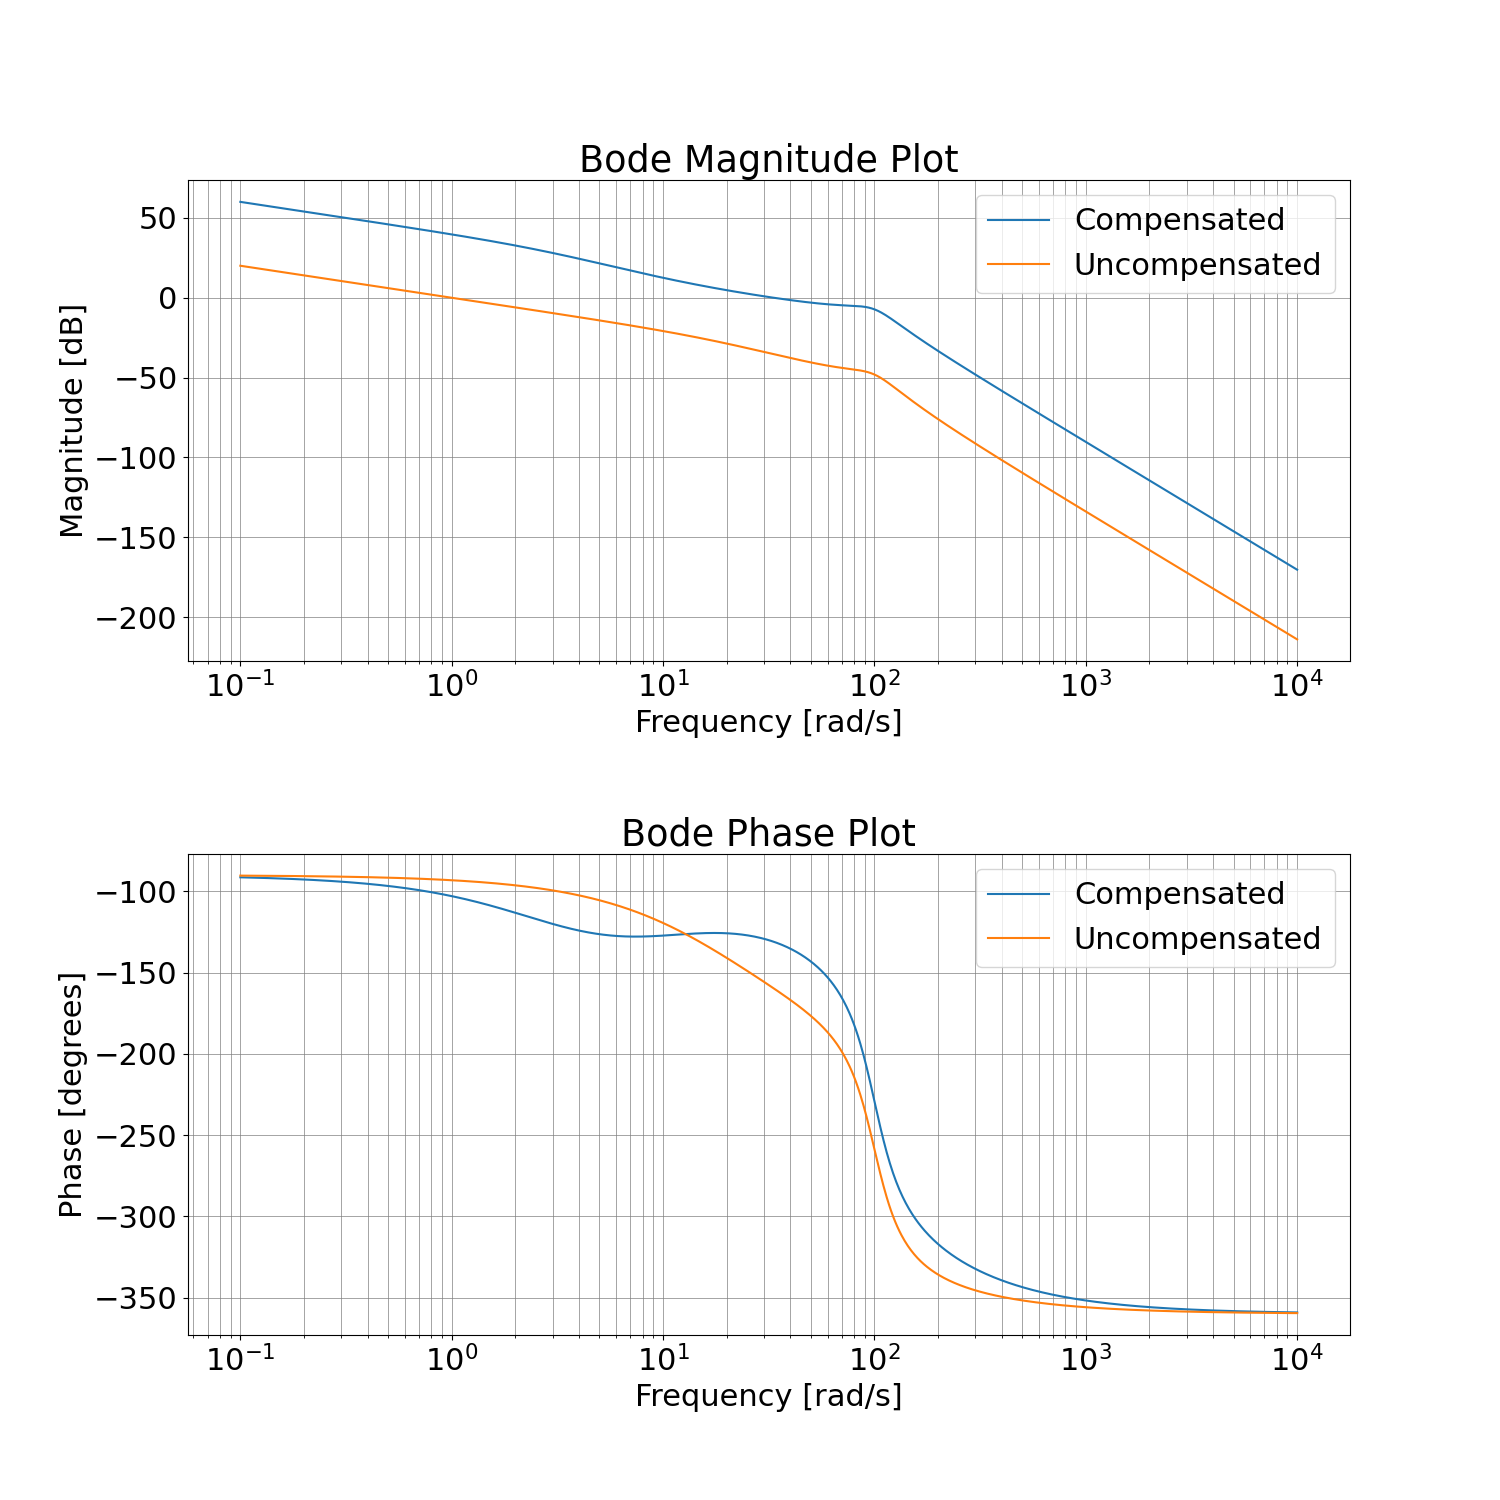
\includegraphics[width=\linewidth]{A4_imgs/q4_bode_final.png}
    \end{center}
    We have $\omega_c = 33.4^\circ$ which is close to $31.6^\circ.$ The inaccuracy is caused by some rounding errors as I only kept two significant digits in some steps. In many applications, this will be an acceptable error since there will always be noise and nonlinearities in the system that will cause the simulation to be inaccurate. 
    \item The phase margin is 
    \begin{equation}
        PM = 48.98^\circ.
    \end{equation}
\end{enumerate}
\newpage
\item \begin{enumerate}[label=(\alph*)]
    \item Let the cascade controller be $D_c(s).$ Then we want $|D_c(j\omega)G(j\omega)| < 0.05$ for $\omega \ge 100$ (shown in red).
    
    Note that we have a type 1 system, so for the steady state error to be smaller than $2\%$ we have $K_v > 1/0.02 = 50$ (Ch6, Part 3, pg 29). The orange region shows the region where this is not satisfied. Note that this itself is an approximation, since it assumes that the gain is very close to its low frequency asymptote at $\omega = 1.$
    
    This is represented below, alongside the Bode plot for the uncompensated system,
    \begin{center}
        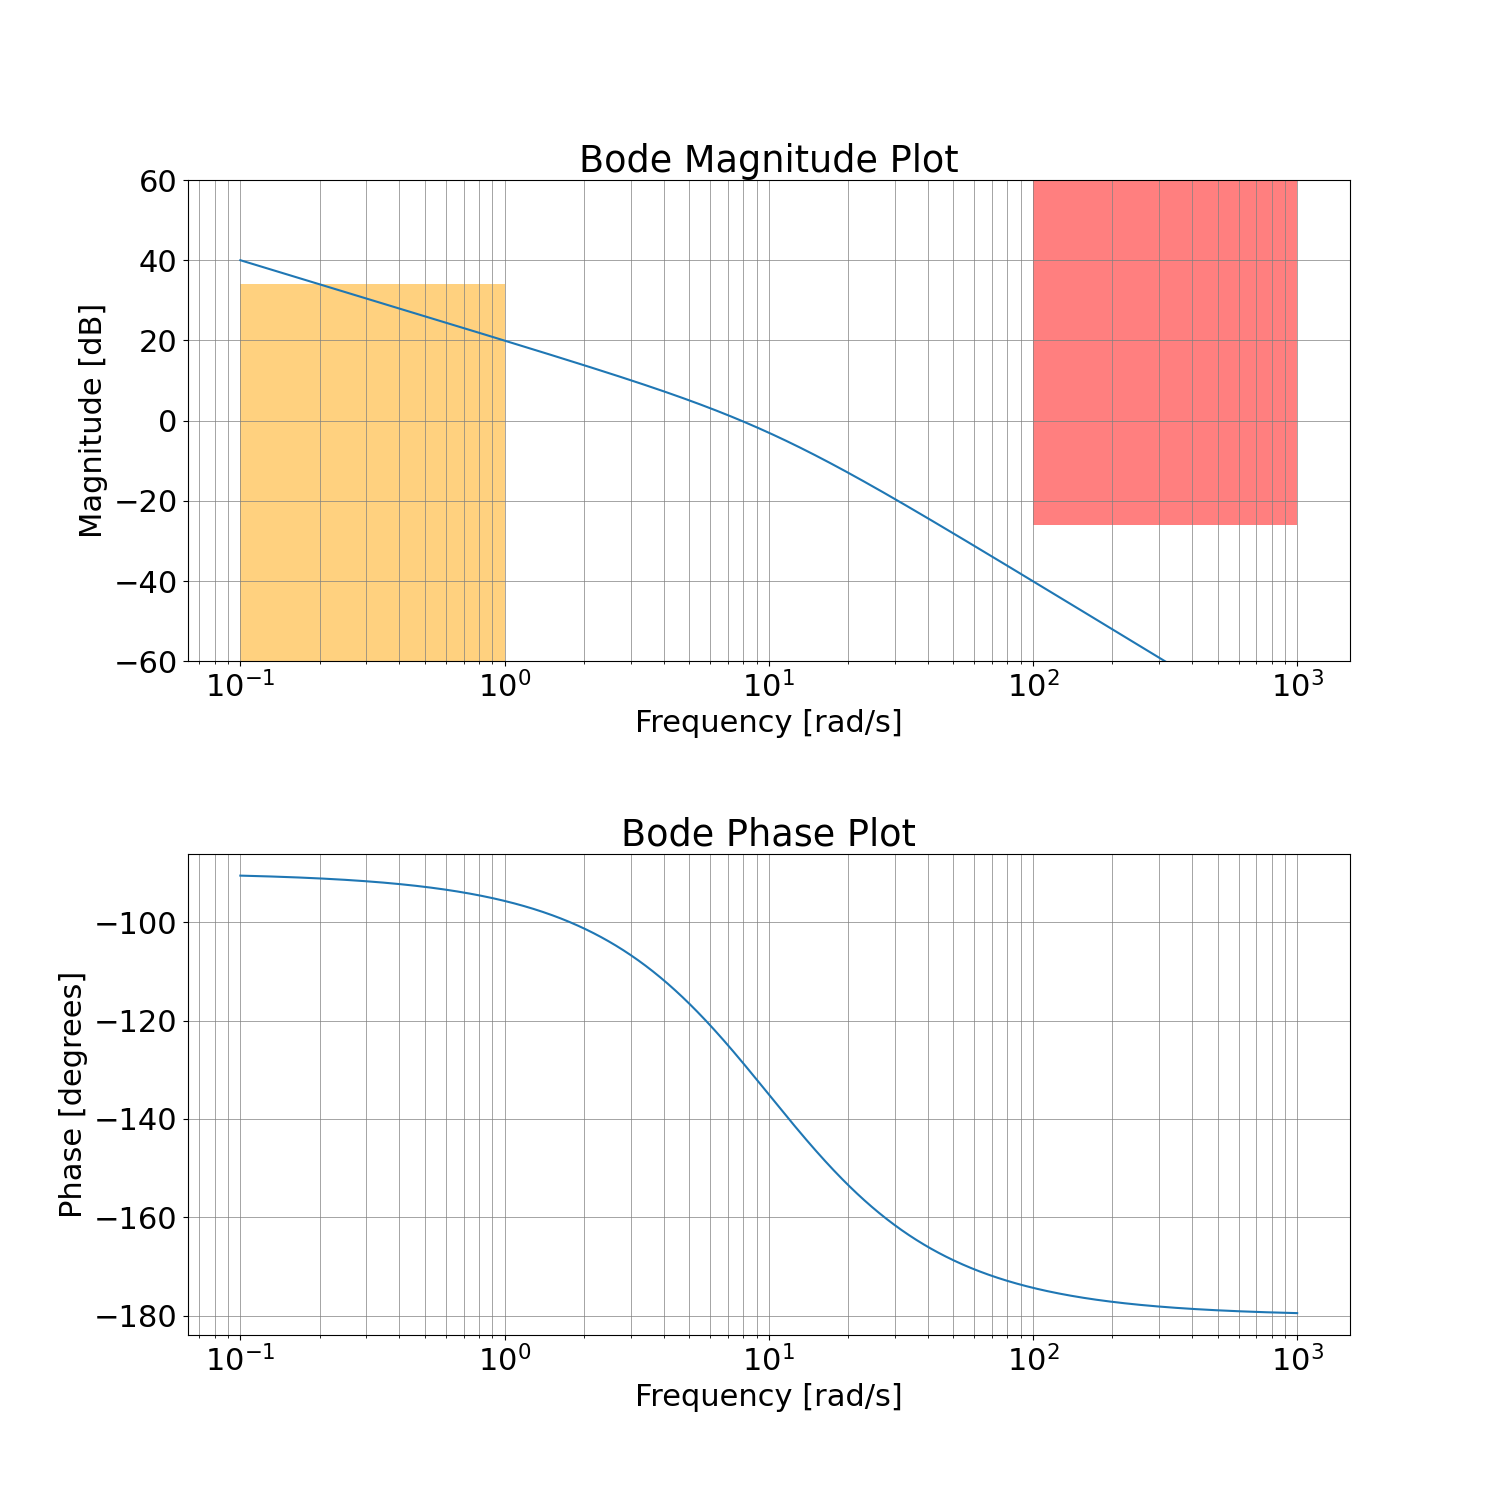
\includegraphics[width=\linewidth]{A4_imgs/q5_bode_nothing.png}
    \end{center}
    \item Note that 
    \begin{equation}
        K_v = \lim_{s\to 0} sKG(s) = 10K
    \end{equation}
    so set $K=10.$ We then get the following Bode plot,
    \begin{center}
        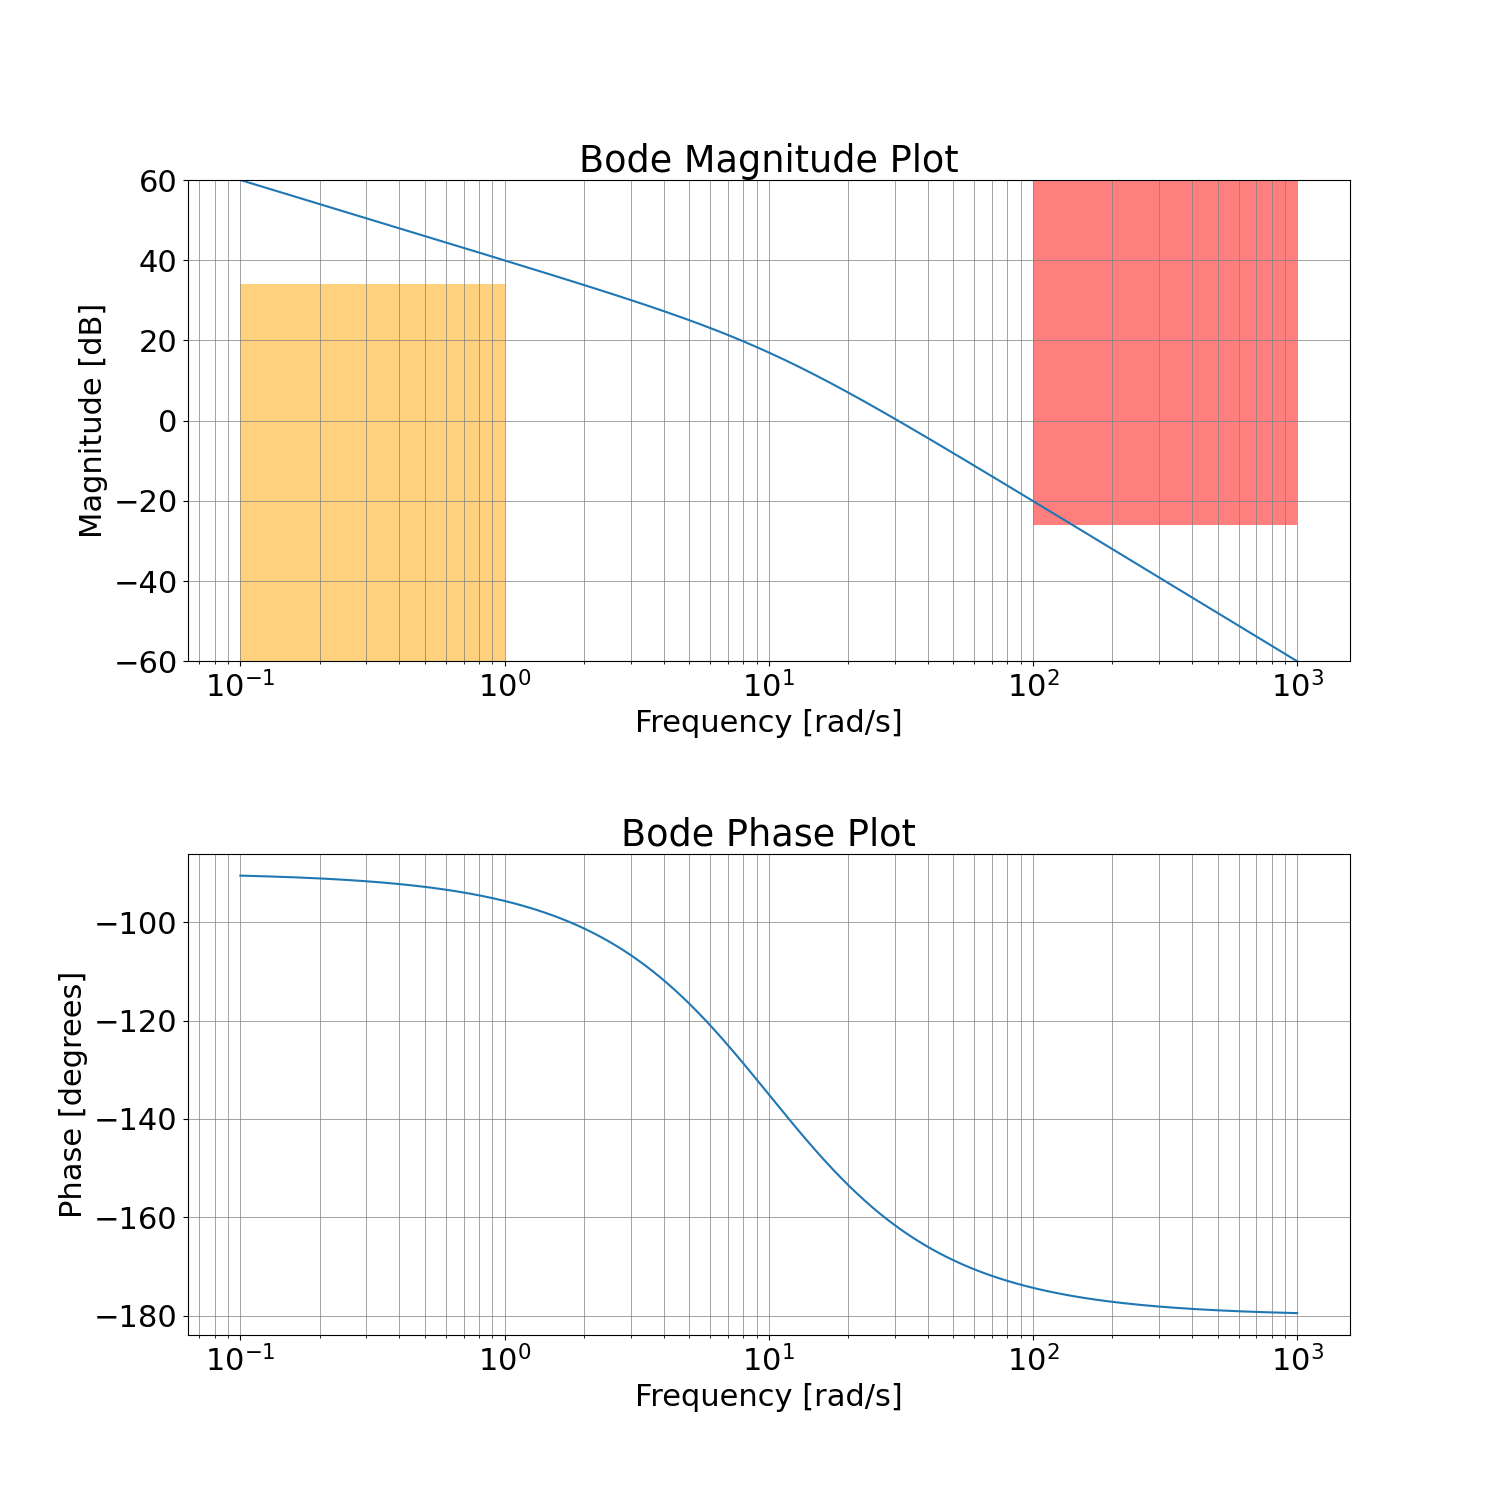
\includegraphics[width=\linewidth]{A4_imgs/q5_bode_b.png}
    \end{center}
    which is not satisfactory. The value of $PM$ is $PM=18^\circ$ which is also not satisfactory. 

    \item Recall that a lag compensator (with unity DC gain) can increase the phase margin, but it would cause the gain to decrease everywhere, as the range is in $(1/\alpha, 1).$ Because the magnitude plot is already near the ``bad regions'' at both the low and high frequencies, it doesn't offer us a lot of flexibility.
    
    Similarly, we can't just use a lead compensator because it'll cause the gain at high frequencies to increase, which is also not desirable.

    So our strategy will be to first use a lag compensator to decrease the gain at high frequencies, which then allows us to use a lead compensator to increase the phase margin. But because higher frequency gains are so far away from the ``bad regions,'' it'll give us a lot of flexibility.
    
    \item Currently, we have $PM=17.9^\circ,$ and we wish to increase it to $55^\circ$ where I added an extra $10^\circ$ for safety. Let's start off with a lag compensator.
    
    We have already determined the DC gain to be unity $K\alpha = 1.$ Similar to problem 2, the magnitude of the lag compensator at high frequencies approaches $\frac{1}{\alpha}.$ Let's make this $-30\text{ dB}$ to be safe, i.e. we have 
    \begin{equation}
        \frac{1}{\alpha} = 10^{-30/20} = 0.1 \implies \alpha = 32.
    \end{equation}
    Pick the upper corner frequency to be a decade below $\omega = 100\text{ rad/s},$ so we can be confident that at this frequency, the magnitude of the plant with the controller is below the red region. Therefore, pick $T_I = 0.1.$ This gives us the controller 
    \begin{equation}
        D_{c,lag} = \frac{0.1s+1}{3.2s+1}.
    \end{equation}
    We get the following Bode plot,
    \begin{center}
        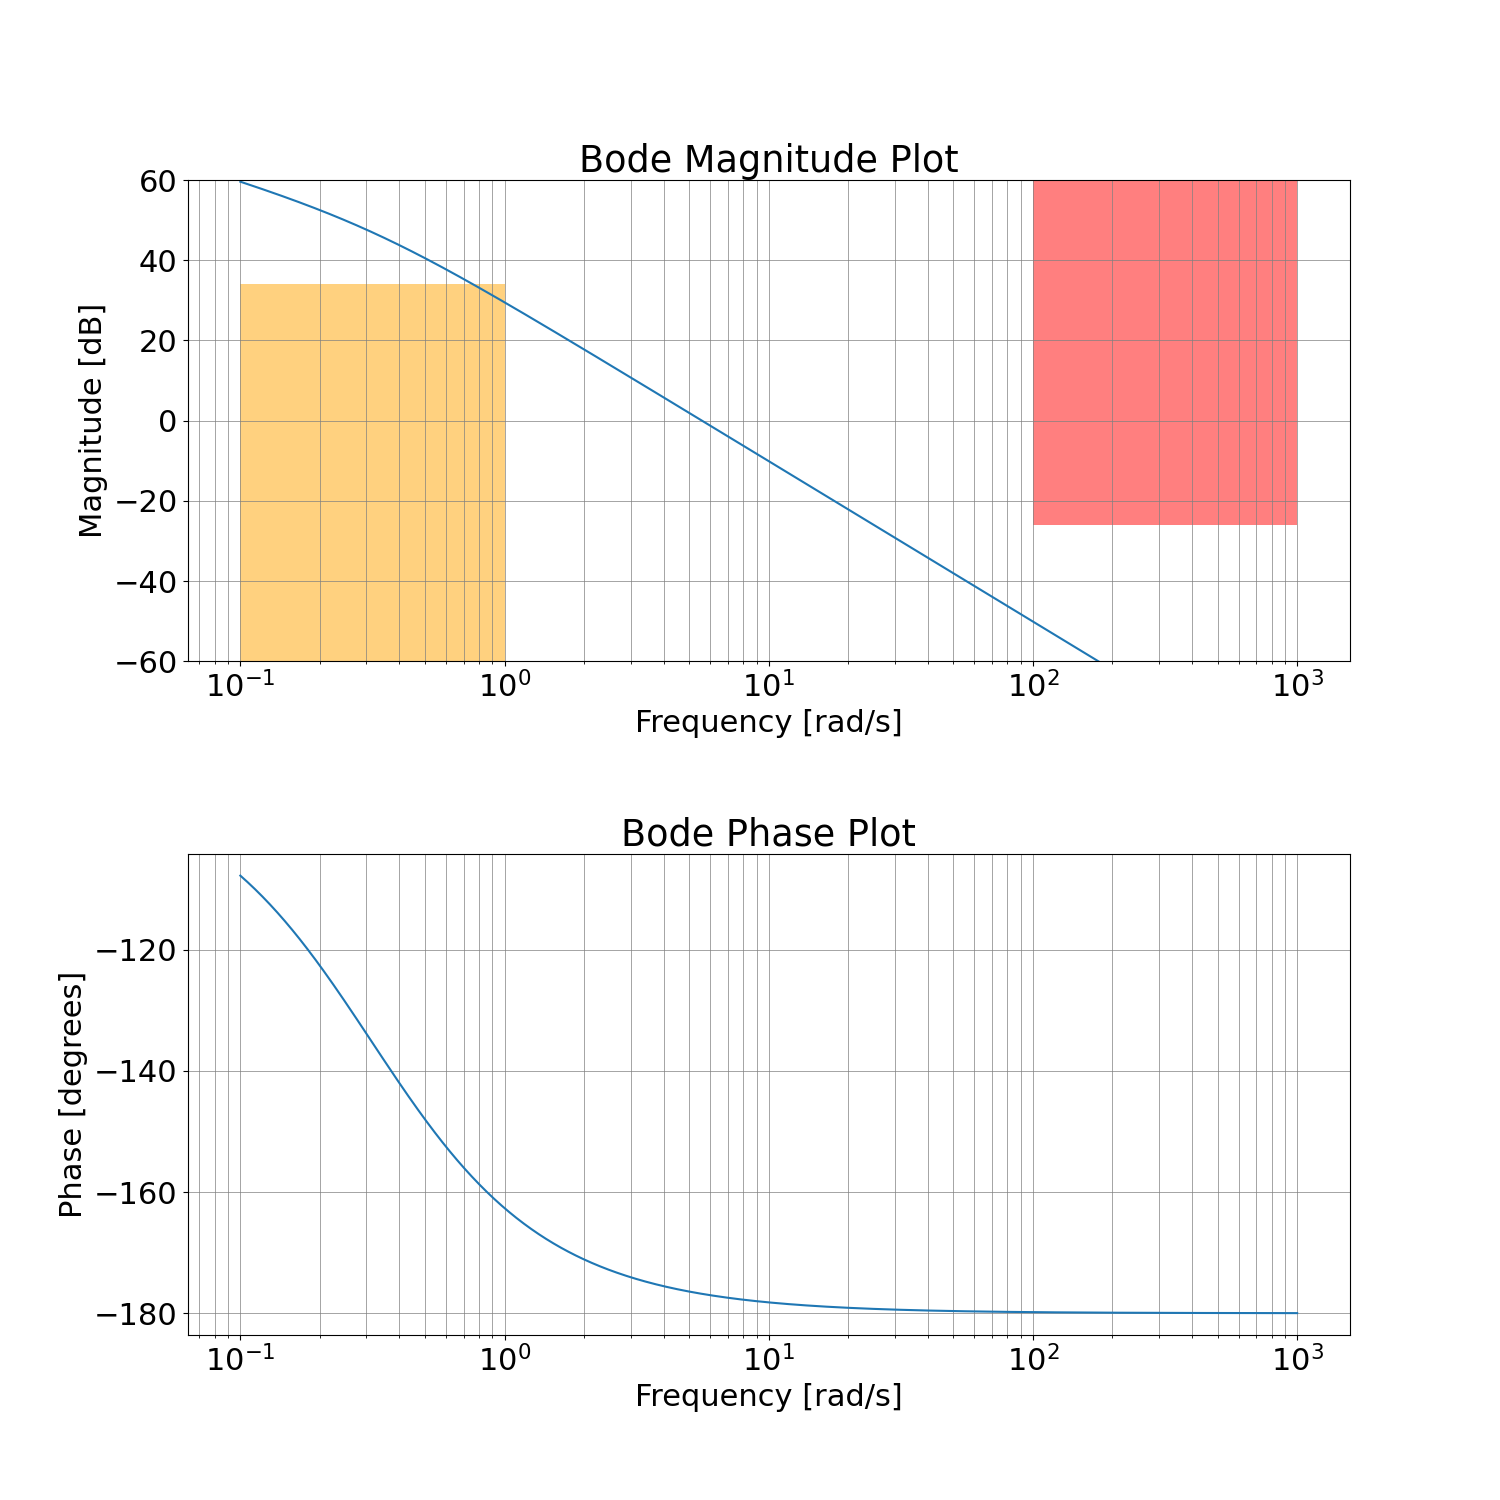
\includegraphics[width=\linewidth]{A4_imgs/q5_bode_d_1.png}
    \end{center}
    where we have $PM = 3.2^\circ.$ Now let's design a lead compensator to increase the phase margin.
    \begin{enumerate}[label=(\arabic*)]
        \item We have already determined that we have $K=1$
        \item $PM=3.2^\circ$
        \item Allow for an extra $10^\circ$ margin for safety, so we want $PM=55^\circ.$ We have 
        \begin{equation}
            \phi_\text{max} = 55 - (3.2) = 52^\circ.
        \end{equation}
        \item Compute 
        \begin{equation}
            \alpha = \frac{1-\sin\phi_\text{max}}{1+\sin\phi_\text{max}} = 0.12.
        \end{equation}
        \item Pick the zero to be at the geometric mean of the two frequencies we're interested in, $\omega=1,100.$ Therefore, $\omega_\text{max}=10\text{ rad/s}$ so 
        \begin{equation}
            T_D = \frac{1}{\omega_\text{max}\sqrt{\alpha}} = 0.29.
        \end{equation}
    \end{enumerate}
    We now get $PM=54^\circ$ and the Bode plot is shown below,
    \begin{center}
        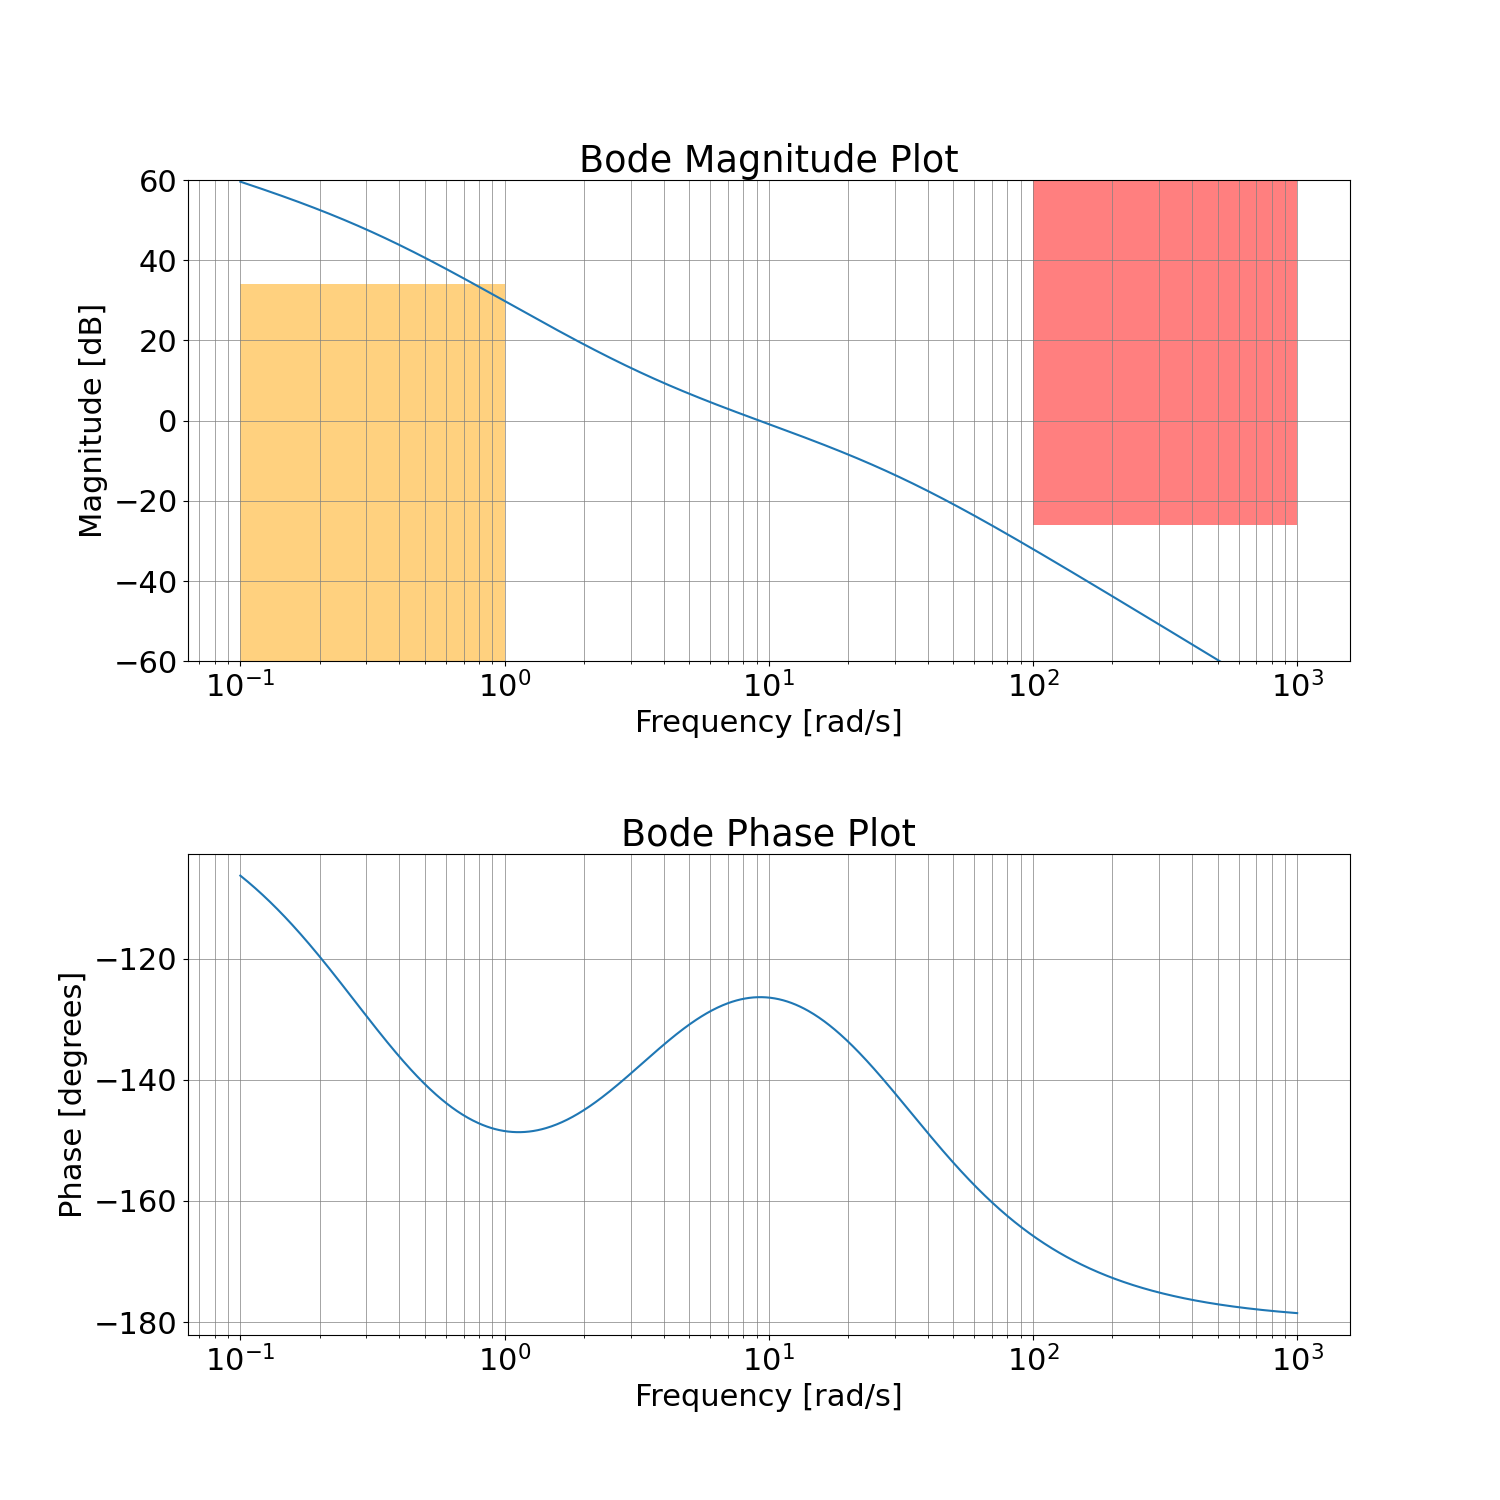
\includegraphics[width=\linewidth]{A4_imgs/q5_bode_d_2.png}
    \end{center}
    However, this intersects the orange region, so we should make some adjustments! The problem comes from choosing a too aggressive $\alpha$ for the lag compensator, which pushed everything down. If we choose $\alpha = 2$ instead, which corresponds to a $-25\text{ dB}$ decrease instead of a $-30\text{ dB}$ decrease, we get the following Bode plot,
    \begin{center}
        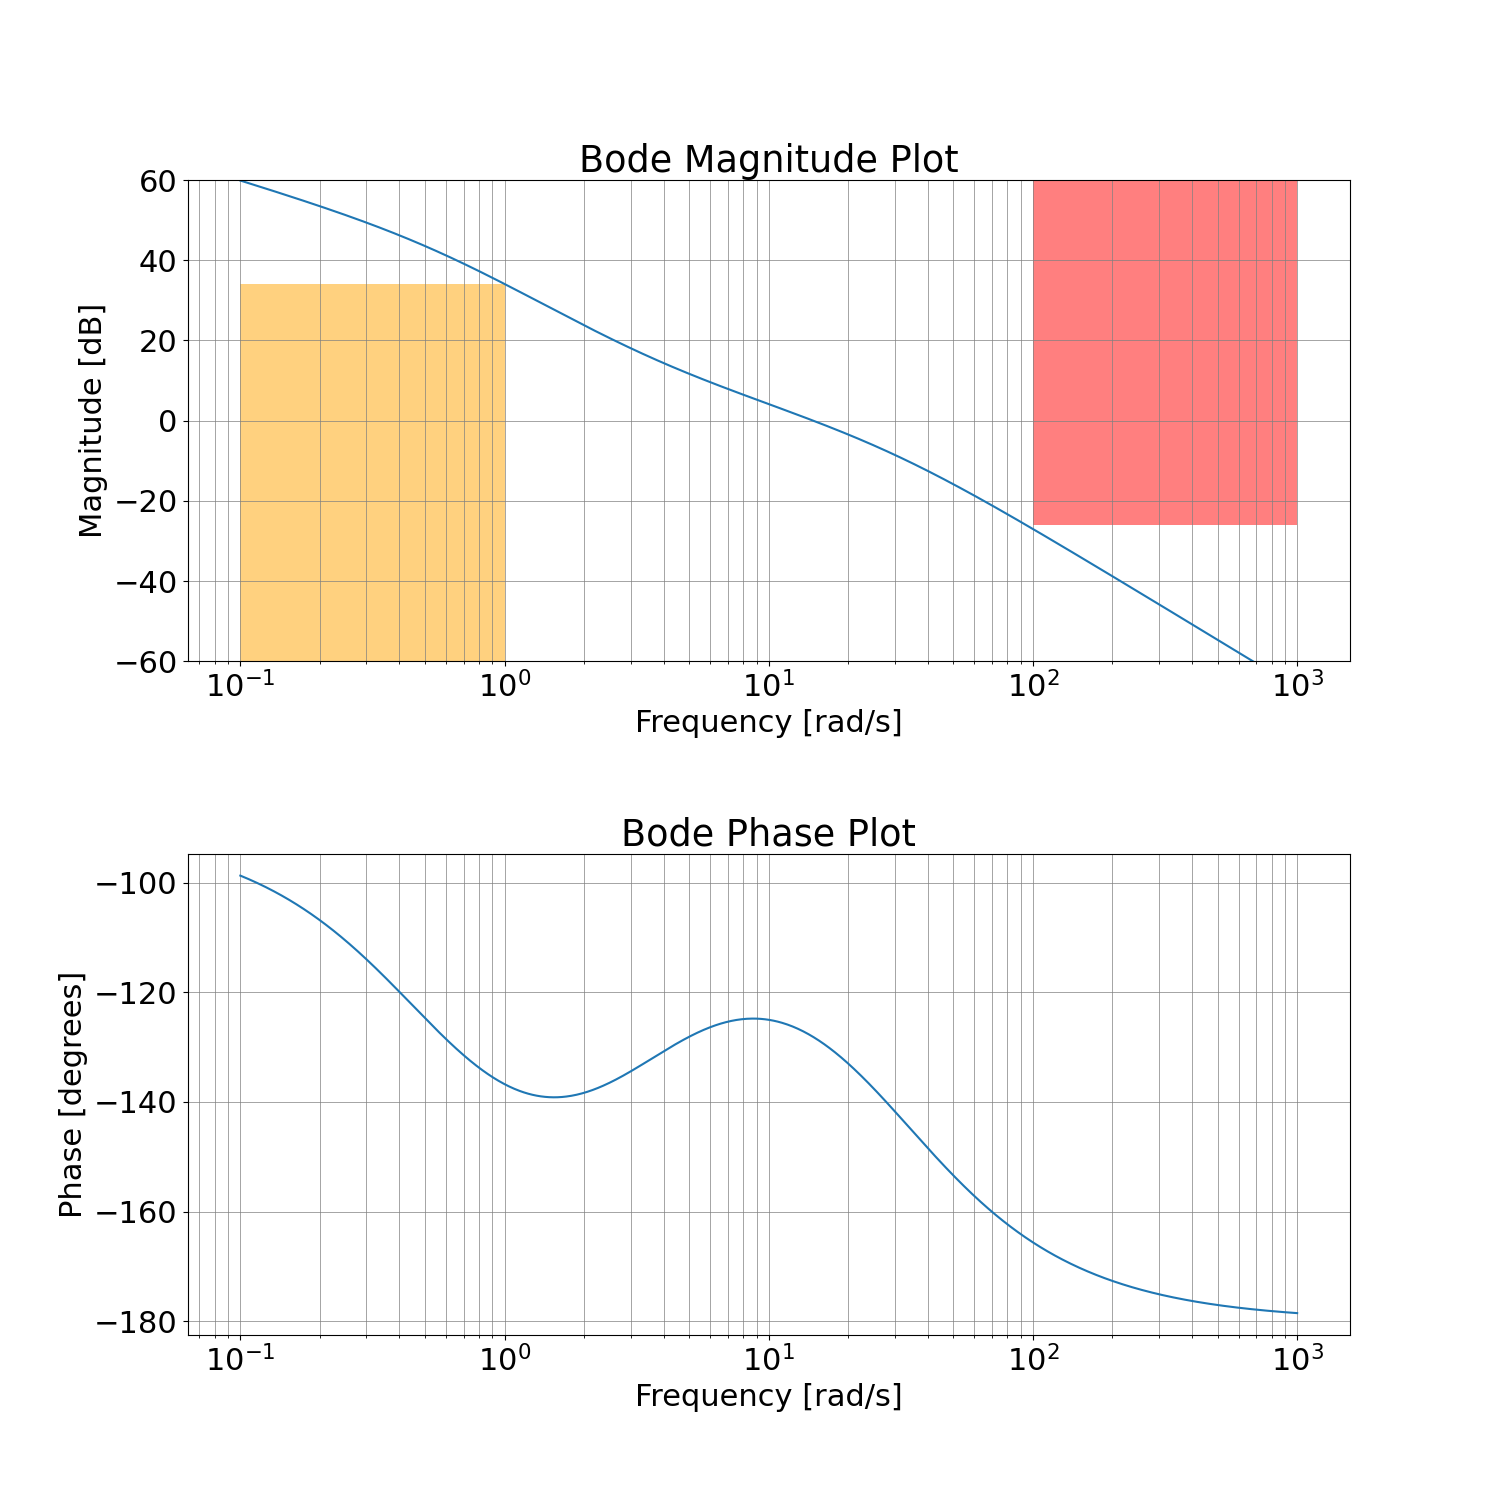
\includegraphics[width=\linewidth]{A4_imgs/q5_bode_d_3.png}
    \end{center}
    which satisfies everything. It has 
    \begin{align}
        PM &=52^\circ \\ 
        mag(\omega=1) &= 34.00 > 20\log_{10}(50) \\ 
        mag(\omega=100) &= -27.14 < 20\log_{10}(0.05).
    \end{align}
    Recall that we said before that the orange region is only an approximation. We actually don't care too much about that in this case since the at $\omega= 1\text{ rad/s}$ we have a gain curve that is slightly concave down, so the actual $K_v$ value at $\omega=1$ will be even higher!

    In conclusion, the final controller is 
    \begin{equation}
        D_c(s) = 10 \cdot \frac{0.1s+1}{1.8s + 1} \cdot \frac{0.29s + 1}{0.0348s + 1}.
    \end{equation}
\end{enumerate}
\end{enumerate}
\appendix
All plots and values were computed using a Python script. The reason I chose to use Python instead of Matlab was because there already was a huge open-source community around signal processing in Python, which is essentially what frequency response / bode plots are, so there are better resources.

There are no huge demands for speed for these tasks, and it's easier to implement an OOP approach that I can later on use and integrate for other projects. The graphs also look much nicer!

% python script
\begin{lstlisting}[language=Python]
import numpy as np
import matplotlib.pyplot as plt
from scipy import signal
import control as ctl

class Bode():
    def __init__(self, G, freq_range = [-2, 2]):
        self.G = G

        # Hacky fix
        # sometimes signal.TransferFunction has better properties
        self.sys = signal.TransferFunction(G.num[0][0], G.den[0][0])

        # Compute frequency response
        self.w, self.mag, self.phase = signal.bode(self.sys, np.logspace(freq_range[0], freq_range[1], 1000))


        # Compute w_BW
        self.w_BW = self.compute_w_BW()

        # Compute w_C
        self.w_C = self.compute_w_C()

        # Compute PM
        self.PM = self.compute_PM()

        # Compute GM
        self.GM = self.compute_GM()

    def __str__(self):
        # Print transfer function
        w_BW_message = 'w_BW = {:.2f} rad/s'.format(self.w_BW)
        w_C_message = 'w_C = {:.2f} rad/s'.format(self.w_C)
        PM_message = 'PM = {:.2f} degrees'.format(self.PM)
        GM_message = 'GM = {:.2f}'.format(self.GM)

        return f'SYSTEM PROPERTIES for {self.G}\n\n' \
                + w_BW_message + '\n' \
                + w_C_message + '\n' \
                + PM_message + '\n' \
                + GM_message
    
    def compute_GM(self):
        ''' 
        Defined as the inverse of |KG(j omega)| when
        angle G(j omega) = -180 degrees
        '''
        try:
            # Find index when phase is -180 degrees
            index = np.where(self.phase < -180)[0][0]

            # Compute the magnitude at this index
            mag = self.mag[index]

            # # convert from dB to linear
            # mag = 10**(mag/20)

            # # Compute GM
            # return 1/mag
            return np.abs(mag)
        except:
            return np.inf

    def w_at_phase(self, phase):
        ''' 
        Defined as the frequency at which the phase of the
        system's frequency response is at a certain phase
        '''
        # Find index of first value that is closest to phase
        index = np.where(self.phase < phase)[0][0]

        # Compute w
        return self.w[index]

    def mag_at_w(self, w):
        ''' 
        Defined as the magnitude of the system's frequency
        response at a certain frequency
        '''
        # Find index of first value that is closest to mag
        index = np.where(self.w > w)[0][0]

        # Compute w
        return self.mag[index]

    def compute_w_C(self):
        '''
        Defined as the frequency at which the magnitude of
        the system's frequency response becomes 0dB
        '''
        try:
            # Find index of first value that is less than 0 dB
            index = np.where(self.mag < 0)[0][0]

            # Compute w_C
            return self.w[index]
        except:
            return np.inf

    def compute_w_BW(self):
        '''
        Defined as frequency at which the magnitude of
        the system's frequency response decreases to -3 dB
        relative to its maximum value
        '''
        # Maximum voltage

        # Find index of first value that is closest to -3 dB

        try:
            index = np.where(self.mag < -3)[0][0]
            return self.w[index]
        except:
            return np.inf
        # Compute w_BW

    def compute_PM(self):
        '''
        The amount by which the phase of G(j omega) exceeds
        -180 deg when |KG(j omega)| = 1.
        '''
        
        try:
            # Find index when magnitude is 0 dB
            index = np.where(self.mag < 0)[0][0]

            # Compute the phase at this index
            phase = self.phase[index]

            # Compute PM
            return phase + 180
        except:
            return np.inf
    
    def plot_bode(self, file_name = None, plot = True):

        # Create a figure
        plt.figure()
        # reset settings
        plt.rcParams.update(plt.rcParamsDefault)

        # make plot bigger
        plt.rcParams["figure.figsize"] = (15,15)

        # make text bigger
        plt.rcParams.update({'font.size': 22})

        # Create Bode magnitude plot (subplot)
        plt.subplot(2, 1, 1)
        plt.semilogx(self.w, self.mag)
        plt.xlabel('Frequency [rad/s]')
        plt.ylabel('Magnitude [dB]')
        plt.title('Bode Magnitude Plot')
        plt.grid(which='both', linestyle='-', linewidth='0.5', color='gray')

        # Create Bode phase plot (subplot)
        plt.subplot(2, 1, 2)
        plt.semilogx(self.w, self.phase)
        plt.xlabel('Frequency [rad/s]')
        plt.ylabel('Phase [degrees]')
        plt.title('Bode Phase Plot')
        plt.grid(which='both', linestyle='-', linewidth='0.5', color='gray')

        plt.subplots_adjust(hspace=0.4)


        # If file_name is not None, save the plot
        if file_name is not None:
            plt.savefig(file_name)

        # Show the plots
        if plot:
            plt.show()
\end{lstlisting}
\end{document}


